\aufgabe{1}{Atomare Axiomenregel}
\newcommand{\Tk}{T_\text{komplex}}
\newcommand{\Ta}{T_\text{atomar}}
Bezeichne $\Tk$ den ursprünglichen Kalkül mit komplexer Axiomenregel $(\phi, \neg \phi, \Gamma / \bot)$ und $\Ta$ den
neuen Kalkül mit atomarer Axiomenregel und sei $\#\phi$ die Anzahl der Konnektive der Formel $\phi$.

N.B.: Außer der Axiomenregel gibt es keine Regel, die \glqq kommaübergreifend\grqq\ arbeitet; dies bedeutet, dass
Regeln, die lediglich auf $\Gamma$ angewendet werden, ignoriert werden können.

Zu zeigen ist, dass $\Ta$ genau dann ein Label $\Gamma$ ablehnt, wenn $\Gamma$ von $\Tk$ abgelehnt wird.

\begin{itemize}
        \item[\glqq$\Rightarrow$\grqq] Lässt sich die atomare Axiomenregel anwenden, so auch die komplexe Axiomenregel.
        \item[\glqq$\Leftarrow$\grqq] Induktion über die Struktur von $\phi$:
                        \paragraph{I.A.} $\#\phi = 0 \Rightarrow \phi = A, A$ Literal $\Rightarrow$ $\Tk$ und $\Ta$ lehnen den
                        Label $\phi, \neg \phi, \Gamma$ ab
                        \paragraph{I.V.} $\forall \phi, \ \#\phi < n$ gelte bereits:
                                \[ \Tk \text{ lehnt } \phi, \neg \phi, \Gamma \text{ ab } \Rightarrow \Ta \text{ lehnt }
                                \phi, \neg \phi, \Gamma \text{ ab } \]
                        \paragraph{I.S.} Seien $\phi_1, \phi_2$ zwei Formeln mit $\#\phi_1 = k_1 < n, \#\phi_2 = k_2 < n$.
                        \begin{itemize}
                                \item[$i)$] $\phi = \phi_1 \wedge \phi_2$ und $\Tk$ lehnt den Label $\phi, \neg \phi, \Gamma$
                                        ab. Folgende Zweige können durch Regelanwendungen im Kalkül $\Ta$ entstehen:

                                        \begin{minipage}{0.4\textwidth}
                                        \begin{prooftree}
                                                \AxiomC{$\phi_1 \wedge \phi_2, \neg (\phi_1 \wedge \phi_2), \Gamma$}
                                                \UnaryInfC{$\phi_1, \phi_2, \neg (\phi_1 \wedge \phi_2), \Gamma$}
                                                \UnaryInfC{$\phi_1, \phi_2, \neg \phi_1, \Gamma$}
                                                \RightLabel{\scriptsize{nach I.V.}}
                                                \UnaryInfC{$\bot$}
                                        \end{prooftree}\end{minipage}\begin{minipage}{0.4\textwidth}
                                        \begin{prooftree}
                                                \AxiomC{$\phi_1 \wedge \phi_2, \neg (\phi_1 \wedge \phi_2), \Gamma$}
                                                \UnaryInfC{$\phi_1, \phi_2, \neg (\phi_1 \wedge \phi_2), \Gamma$}
                                                \UnaryInfC{$\phi_1, \phi_2, \neg \phi_2, \Gamma$}
                                                \RightLabel{\scriptsize{nach I.V.}}
                                                \UnaryInfC{$\bot$}
                                        \end{prooftree}
                                        \end{minipage}

                                    In beiden Fällen wird der Label auch von $\Ta$ abgelehnt.

                                \item[$ii)$] $\phi = \neg\phi_1$ und $\Tk$ lehnt den Label $\neg\phi_1, \neg\neg\phi_1, \Gamma$
                                        ab. Im Kalkül $\Ta$ erhält man:
                                        \begin{prooftree}
                                                \AxiomC{$\neg\phi_1, \neg\neg\phi_1, \Gamma$}
                                                \RightLabel{\scriptsize{$(\neg\neg)$}}
                                                \UnaryInfC{$\neg\phi_1, \phi_1, \Gamma$}
                                                \UnaryInfC{$\bot$}
                                        \end{prooftree}

                                    Der Label wird also auch von $\Ta$ abgelehnt.
                        \end{itemize}
                        Da es nur die Konnektive $\wedge$ und $\neg$ gibt, folgt die Behauptung.
\end{itemize}

\newpage
\aufgabe{2}
Da der Label $\Gamma$ endlich viele Konnektive hat und jede Regel die Anzahl der Konnektive verringert, führen alle
Kombinationen von Regelanwendungen in endlicher Zeit zur Terminierung. Damit ist der Begriff eines \emph{erfolgreichen}
Labels wohldefiniert.

Der Begriff \emph{erfolgreich} wird also verallgemeinert, sodass ein Baum von Regelanwendungen entsteht, bei dem die
Pfade von der Wurzel zu jedem Blatt Folgen von Regelanwendungen repräsentieren, deren Anwendungen auf $\Gamma$ zu einer
erfolgreichen Terminierung des Tableaualgorithmus führen.

Zu zeigen: Label erfolgreich $ \ \Leftrightarrow \ \exists $ erfolgreicher Zweig
Beweis:
\begin{itemize}
        \item [$\Rightarrow$] Nach Definition.
        \item [$\Leftarrow$] Label $\Gamma$ hat im Tableaualgorithmus einen erfolgreichen Zweig.
                
                Induktion über die Baumhöhe:
                \paragraph{I.A.} Höhe 0: $\Gamma = A_1, \dots, A_m$, $A_i$ verschiedene Literale (negativ oder positiv),
                d.h. es ist keine weitere Regel anwendbar $\Rightarrow \ \Gamma$ erfolgreich (\emph{vacuously}).
                \paragraph{I.V.} Für alle Label $\Gamma$ der Höhe $k < n$ mit erfolgreichem Zweig gelte die Behauptung.
                \paragraph{I.S.} Höhe $n$.
                \begin{itemize}
                        \item[$(\wedge)$] $\Gamma = \varphi \wedge \psi, \Xi \ \vdash \ \phi, \psi, \Xi \ \Rightarrow $ Höhe
                                $< n$

                                Nach I.V. gilt: $\varphi, \psi, \Xi$ ist erfolgreicher Label. Somit führt auch
                                die Regelanwendung bei $\Gamma$ zu einer erfolgreichen Konklusion.
                        \item[$(\neg\neg)$] $\Gamma = \neg \neg \varphi, \Xi \ \vdash \ \varphi, \Xi \ \Rightarrow $ Höhe
                                $< n$

                                Nach I.V. gilt: $\varphi, \Xi$ ist erfolgreicher Label. Somit führt auch
                                die Regelanwendung bei $\Gamma$ zu einer erfolgreichen Konklusion.
                        \item[$(\neg\wedge)$] $\Gamma = \neg (\varphi \wedge \psi), \Xi \ \vdash \ \neg \varphi, \Xi \|
                                \neg \psi, \Xi \ \Rightarrow $ Höhe jeweils
                                $< n$

                                O.B.d.A. ist $\neg \varphi, \Xi$ erfolgreicher Zweig von $\Gamma$. Nach I.V. gilt:
                                $\neg \varphi, \Xi$ ist erfolgreicher Label. Somit führt auch diese Regelanwendung bei
                                $\Gamma$ zu mindestens einer erfolgreichen Konklusion.
                \end{itemize}
                Somit hat $\Gamma$ für jede mögliche Regelanwendung eine erfolgreiche Konklusion.
\end{itemize}
Damit ist $\Gamma$ ein erfolgreicher Label.

\newpage
\aufgabe{3}{Reduktion von BDDs}
Die Formel $(x \vee y) \wedge (z \vee w)$ kann dargestellt werden als baumförmiges BDD:

\begin{center}
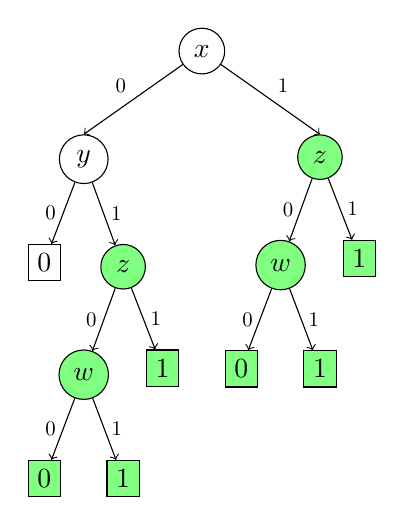
\begin{tikzpicture}[
        nterm/.style={circle,draw,anchor=north},
        term/.style={rectangle,draw,anchor=north},
        level distance=0.76cm, growth parent anchor=south, sibling distance=3cm
        ]
        \node (x) [nterm] {$x$} [->]
            child{ [sibling distance=1cm] node (y) [nterm] {$y$}
            child{ node (a0) [term] {$0$} edge from parent node[left,scale=.75] {$0$} }
                        child{ node (z1) [nterm,fill=green!50] {$z$}
                                    child{ node (w1) [nterm,fill=green!50] {$w$}
                                                child{ node (b0) [term,fill=green!50] {$0$} edge from parent node[left,scale=.75] {$0$} }
                                                child{ node (a1) [term,fill=green!50] {$1$} edge from parent node[right,scale=.75] {$1$} }
                                    edge from parent node[left,scale=.75] {$0$} }
                                    child { node (b1) [term,fill=green!50] {$1$} edge from parent node[right,scale=.75] {$1$} }
                        edge from parent node[right,scale=.75] {$1$} }
            edge from parent node[above left,scale=.75] {$0$} }
            child{ [sibling distance=1cm] node (z2) [nterm,fill=green!50] {$z$}
                        child{ node (w2) [nterm,fill=green!50] {$w$}
                                    child{ node[fill=green!50] (c0) [term] {$0$} edge from parent node[left,scale=.75] {$0$} }
                                    child{ node[fill=green!50] (c1) [term] {$1$} edge from parent node[right,scale=.75] {$1$} }
                               edge from parent node[left,scale=.75] {$0$} }
                        child{ node (d1) [term,fill=green!50] {$1$} edge from parent node[right,scale=.75] {$1$} }
        edge from parent node[above right,scale=.75] {$1$} };
\end{tikzpicture}
\end{center}

Die farbig markierten Untergraphen der beiden $z$-Knoten sind isomorph. Somit kann einer der $z$-Knoten entfernt werden,
wobei die eingehende Kante auf den anderen $z$-Knoten umgebogen wird. Dadurch entsteht der links abgebildete Graph:

\begin{minipage}{0.4\textwidth}
\begin{center}
\begin{tikzpicture}[
        p/.style={scale=.75,->,draw},
        nterm/.style={circle,draw,anchor=north},
        term/.style={rectangle,draw,anchor=north},
        level distance=0.76cm, growth parent anchor=south, sibling distance=2cm
        ]
        \node (x) [nterm] {$x$};
        \node [nterm,below left=of x] (y) {$y$};
        \node [nterm,below right=of x] (z) {$z$};
        \node [term,below left=of y,fill=red!50] (a0) {$0$};
        \node [nterm,below left=of z] (w) {$w$};
        \node [term,below right=of z,fill=blue!50] (a1) {$1$};
        \node [term,below left=of w,fill=red!50] (b0) {$0$};
        \node [term,below right=of w,fill=blue!50] (b1) {$1$};
        \path [p] (x) -- node[above left] {$0$} (y);
        \path [p] (x) -- node[above right] {$1$} (z);
        \path [p] (y) -- node[above left] {$0$} (a0);
        \path [p] (y) -- node[above] {$1$} (z);
        \path [p] (z) -- node[above left] {$0$} (w);
        \path [p] (z) -- node[above right] {$1$} (a1);
        \path [p] (w) -- node[above left] {$0$}  (b0);
        \path [p] (w) -- node[above right] {$1$}  (b1);
\end{tikzpicture}
\end{center}
\end{minipage}\hfill\begin{minipage}{0.4\textwidth}
\begin{center}
\begin{tikzpicture}[
        p/.style={scale=.75,->,draw},
        nterm/.style={circle,draw,anchor=north},
        term/.style={rectangle,draw,anchor=north},
        level distance=0.76cm, growth parent anchor=south, sibling distance=2cm
        ]
        \node (x) [nterm] {$x$};
        \node [nterm,below left=of x] (y) {$y$};
        \node [nterm,below right=of x] (z) {$z$};
        \node [nterm,below left=of z] (w) {$w$};
        \node [term,below left=of w,fill=red!50] (b0) {$0$};
        \node [term,below right=of w,fill=blue!50] (b1) {$1$};
        \path [p] (x) -- node[above left] {$0$} (y);
        \path [p] (x) -- node[above right] {$1$} (z);
        \path [p] (y) -- node[left] {$0$} (b0);
        \path [p] (y) -- node[above] {$1$} (z);
        \path [p] (z) -- node[above left] {$0$} (w);
        \path [p] (z) -- node[right] {$1$} (b1);
        \path [p] (w) -- node[above left] {$0$}  (b0);
        \path [p] (w) -- node[above right] {$1$}  (b1);
\end{tikzpicture}
\end{center}
\end{minipage}

Nach Entfernen der doppelten terminalen Knoten erhält man den rechten Graphen, das vollständig reduzierte BDD.

\aufgabe{4}{Erfüllbarkeit von BDDs}
Ein BDD ist erfüllbar, wenn es einen Pfad von der Wurzel $r$ zu einem Terminal mit Label $1$ gibt. Die Existenz eines
terminalen Knotens mit Label $1$ ist sogar hinreichend:

Gäbe es einen terminalen Knoten $1$ ohne, dass ein Pfad von der Wurzel zu ihm existiert, so gäbe es außer der Wurzel
mindestens noch einen initialen Knoten, was im Widerspruch zur Definition eines BDD steht.

$\Rightarrow$ Algorithmus: Durchsuchen der Knotenmenge nach terminalem Knoten mit Label $1$. Die Laufzeit ist linear in
der Länge der Eingabe, der Algorithmus arbeitet ohne Platzoverhead.
